% 本文件是示例论文的一部分
% 论文的主文件位于上级目录的 `main.tex`

\chapter{YOLO算法理论及数据集预处理}

\section{YOLOv11网络结构}
YOLOv11的网络架构采用骨干网络-颈部网络-检测头的分层设计。骨干网络作为特征提取的基石,引入C3K2模块、SPPF(快速空间金字塔池化)和C2PSA(具有注意力机制的卷积模块)组件,实现了高效的底层特征提取;颈部网络将C2F模块替换为了C3K2模块,提升了特征聚合过程的整体性能,通过C2PSA模块增强了对空间注意力机制的关注;检测头负责生成目标检测和分类的最终预测,它处理从颈部网络传递过来的特征图,最终输出图像中目标的边界框和类别标签。\ref{fig:s}(图像来源:\url{https://zhuanlan.zhihu.com/p/4251780251})展示了YOLOv11的网络结构。
\begin{figure}[!htb]
  \centering
  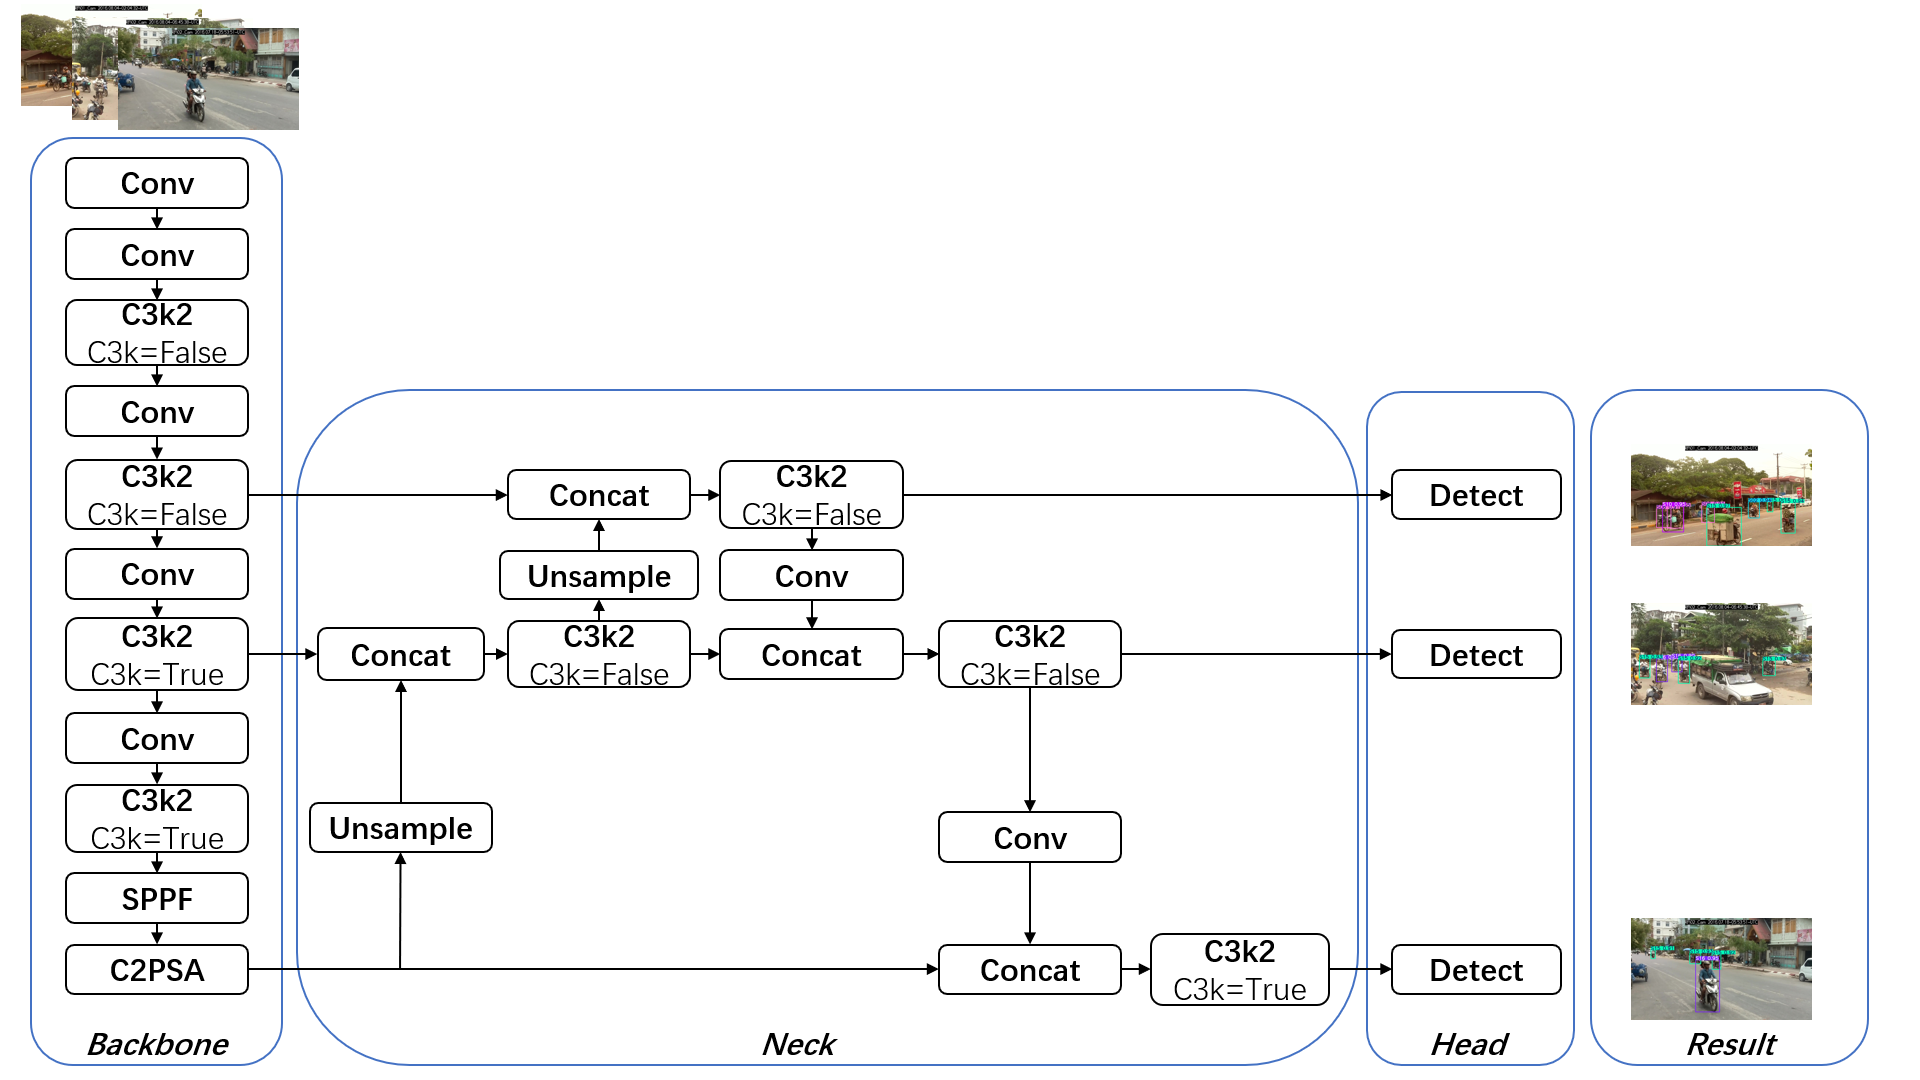
\includegraphics[width=1\textwidth]{figs/chap02/yolov11.png}
  \caption{YOLOv11网络模型}
  \label{fig:s}
\end{figure}

\subsection{骨干网络}
YOLOv11的骨干网络是整个架构的核心特征提取模块,包含Conv、C3K2、SPPF和C2PSA模块。

Conv卷积模块的处理步骤可以概括为数据准备、参数配置、卷积运算和非线性激活四步。Conv模块的输入通常是$(B, C, W, H)$四维张量,$B$表示训练批次;$C$表示数据通道数,彩色RGB图像的通道数为3;$W$表示图像的宽度,$H$表示高度。卷积层的核心参数包括卷积核、步长(stride)、填充(padding),卷积核决定特征提取的局部感知范围,步长控制卷积核滑动间隔以实现下采样,填充通过边界补零调整输出尺寸以及输出通道数。卷积运算这一步将配置好的卷积核应用于输入数据,通过滑动窗口对每个局部区域进行加权求和,实现特征提取。非线性激活应用ReLU、silu等激活函数引入非线性变换,使模型能够学习复杂模式,最终输出处理后的特征图用于后续层的计算。

C3K2模块是早期版本中引入的CSP(Cross Stage Partial) Bottleneck的演变,用来处理骨干网络不同阶段的特征提取。C3K2模块通过分割特征图,并应用一系列较小的(3$\times$3)卷积核进行卷积操作,优化了网络中的信息流,这些卷积比较大的卷积核更快,计算成本更低。与YOLOv8的C2F模块相比,C3K2模块能够以更少的参数提升特征表示能力。
C3K2模块使用C3K模块来处理信息。它在开始和结束时各有一个Conv模块,中间是一系列的C3K模块。将起始Conv模块的输出与最后一个C3K模块的输出进行拼接,并以一个最终的Conv模块结束。这个模块借助CSP结构,致力于在速度和准确性之间保持平衡。
C3K模块的结构与C2F模块类似,但在此模块中不会进行分割操作。输入数据先经过一个卷积模块,随后经过一系列Bottleneck,并以最终的Conv块结束。这三个模块的结构如\ref{fig:c3k}(图像来源:\url{https://medium.com/@nikhil-rao-20/yolov11-explained-next-level-object-detection-with-enhanced-speed-and-accuracy-2dbe2d376f71})所示。

\begin{figure}[!htb]
  \centering
  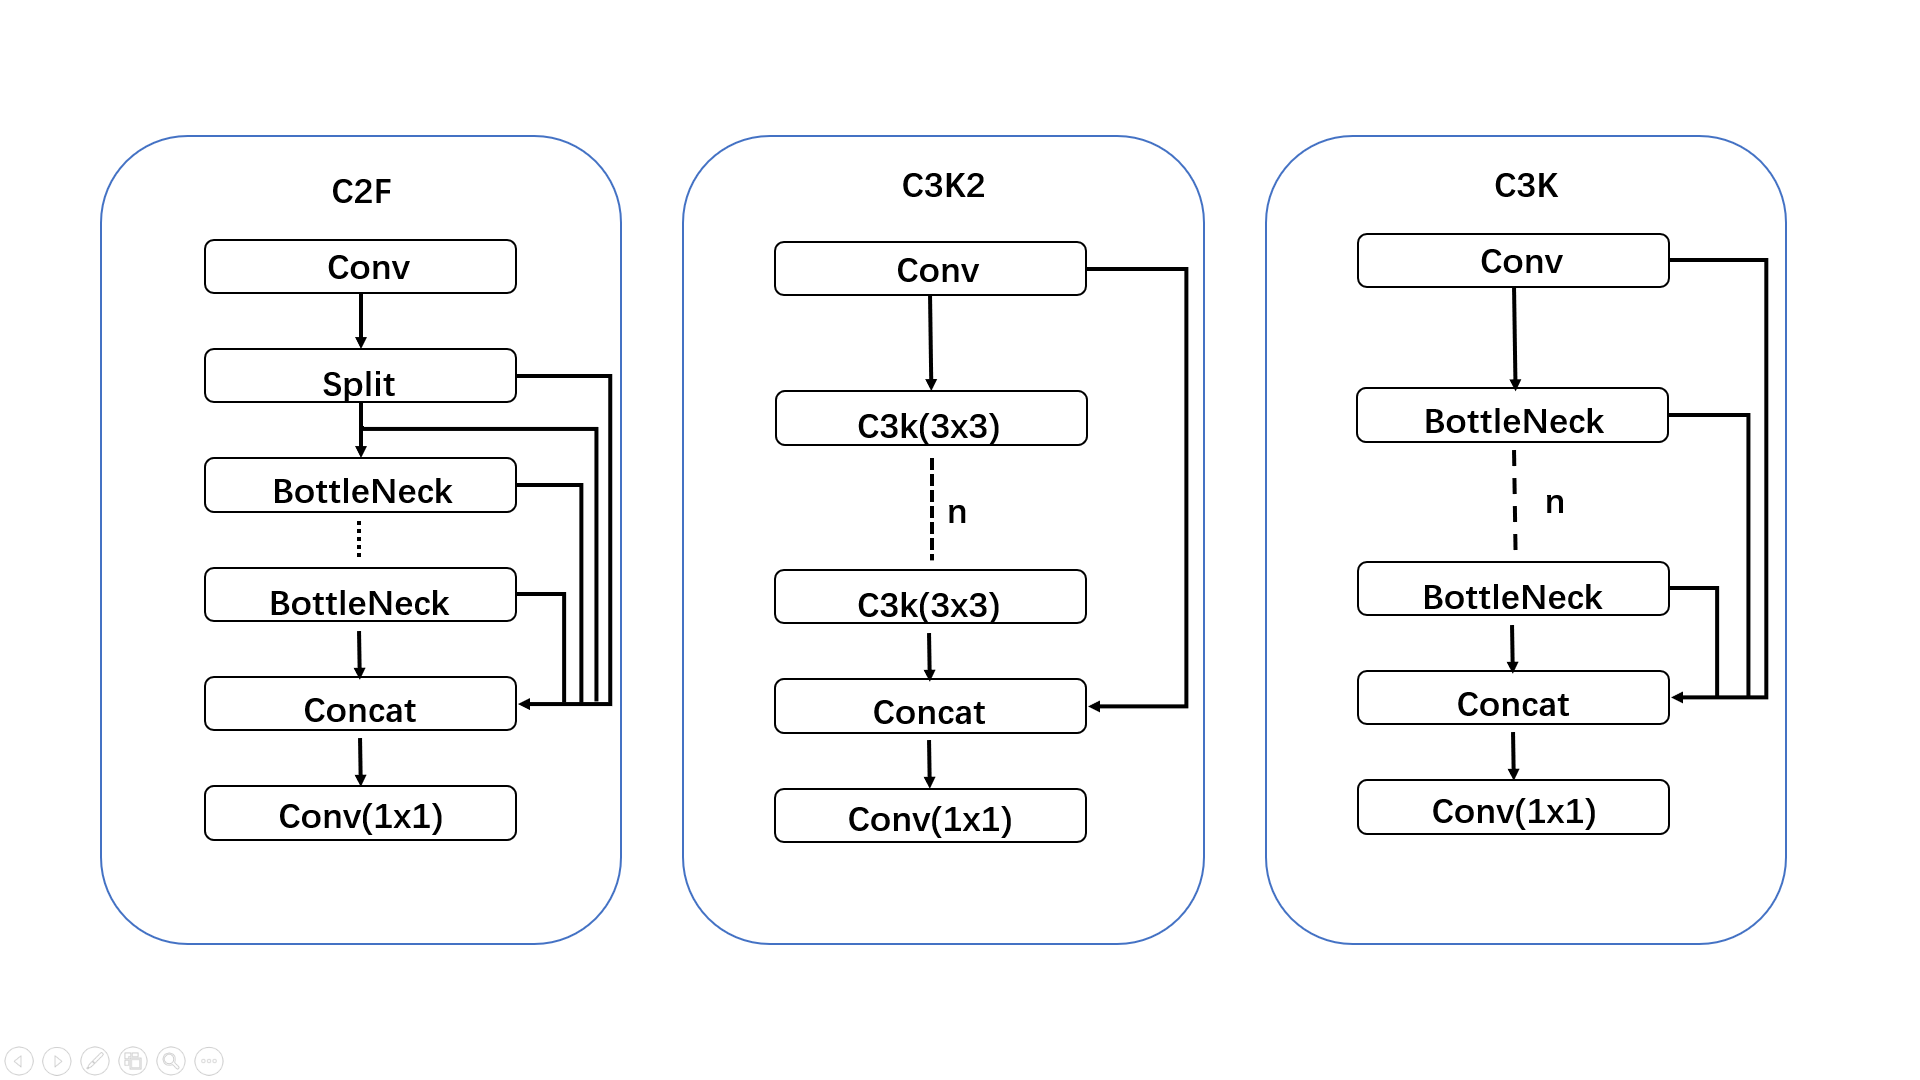
\includegraphics[width=0.9\textwidth]{figs/chap02/c2f.png}
  \caption{C2F和C3K2模块的比较}
  \label{fig:c3k}
\end{figure}

SPPF(Spatial Pyramid Pooling - Fast)模块是对SPP(Spatial Pyramid Pooling)模块的改进,主要用于增强模型对不同尺度目标的检测能力,其结构如\ref{fig:sppf}(图像来源:\url{https://zhuanlan.zhihu.com/p/4251780251})所示。SPPF模块接收C3K2模块输出的特征图,对特征图同时应用多个不同大小的最大池化操作(MaxPool),然后将原始特征图和所有池化后的特征图在通道维度上拼接,形成更丰富的多尺度特征表示,最后通过1×1卷积压缩拼接后的特征通道数,减少计算量。

\begin{figure}[!htb]
  \centering
  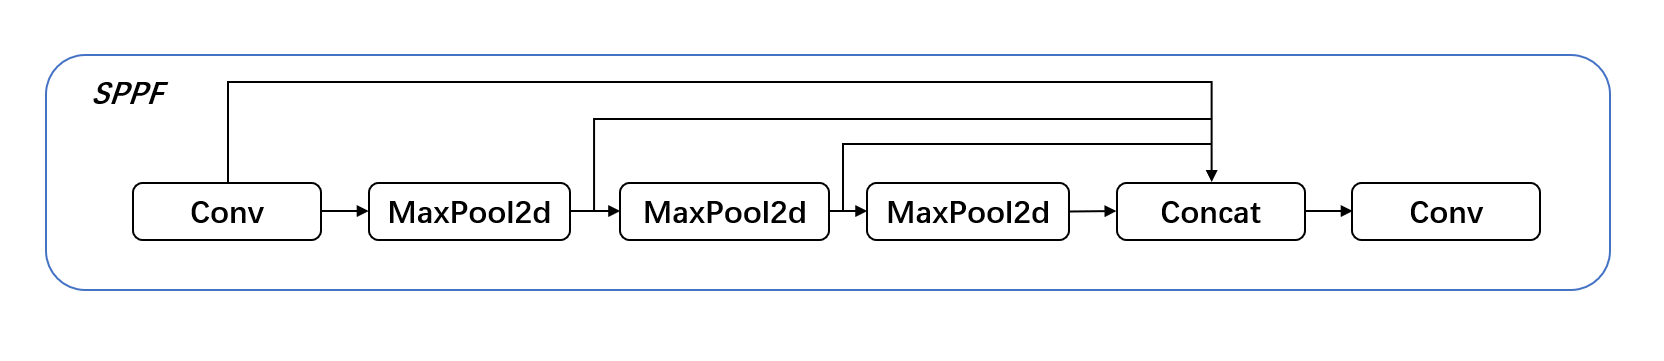
\includegraphics[width=0.9\textwidth]{figs/chap02/sppf.png}
  \caption{SPFF模块结构}
  \label{fig:sppf}
\end{figure}

该模块采用多尺度最大池化核进行特征提取,有效实现对目标多尺度特征的全面表征,通过对不同尺寸池化核获取的特征图进行整合。

C2PSA模块是YOLOv11的一大创新点,该模块结构如\ref{fig:c2psa}(图像来源:\url{https://zhuanlan.zhihu.com/p/4251780251})所示。此模块引入了注意力机制,提高模型对图像中重要区域(例如较小或部分遮挡的对象)的关注。C2PSA模块中的Position-Sensitive Attention封装了对输入张量应用位置敏感注意力和前馈网络的功能,提升了特征提取和处理能力。C2PSA模块采用两个PSA(Partial Spatial Attention)模块,分别处理特征图分支后再拼接,类似C2F模块结构。这种设置在兼顾计算成本与检测精度的同时,让模型聚焦空间信息,使YOLOv11在需关注物体细节以实现精确检测的场景中优于YOLOv8等版本。

\begin{figure}[!htb]
  \centering
  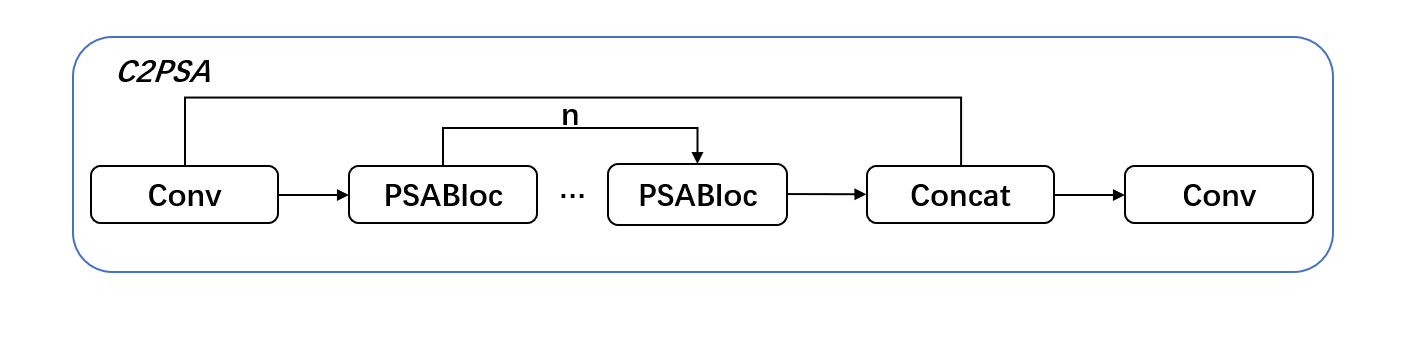
\includegraphics[width=0.9\textwidth]{figs/chap02/c2psa.png}
  \caption{C2PSA模块结构}
  \label{fig:c2psa}
\end{figure}

\subsection{颈部网络}
颈部网络由多个Conv卷积层、C3K2模块、Concat操作和上采样模块组成,并结合了C2PSA机制的优势。

Conv模块对特征图进行卷积运算,一方面可以调整特征图的通道数,使不同特征图在拼接前通道数匹配;另一方面能进一步提取特征,增强特征表达。C3K2模块应用了一系列较小的卷积核,以更少的参数提升特征表示能力。Concat模块沿着通道维度将多个特征图合并在一起,融合不同尺度的特征信息,增加特征的丰富度。
上采样模块通过运用插值等技术手段,实现特征图尺寸的扩充。这一操作的核心目的在于确保特征图维度与其他分支保持一致,借助这种方式,模型得以充分融合多尺度特征信息,提升了模型的检测精度。

颈部网络接收骨干网络不同层级输出的特征图,一些特征图会先经过Unsample上采样操作,使其尺寸与其他待拼接特征图一致,然后再进行Concat拼接。拼接后的特征图,再次经过若干C3K2模块和Conv卷积层,进一步融合与提炼特征。

\subsection{检测头}
与早期的YOLO版本类似,YOLOv11使用多尺度预测头来检测不同大小的对象。头部使用由主干网络和颈部网络生成的特征映射输出三种不同比例(低、中、高)的检测框。
检测头会输出来自三个特征映射(通常来自P3、P4和P5)的预测,对应于图像中的不同尺度级别。这种方法可以确保在更精细的细节(P3)中检测到较小的对象,而在更高级别的特征(P5)中捕获较大的对象​。

\section{YOLOv11损失函数}
YOLOv11的损失函数主要分为:边界框回归损失(BBox Loss)、分类损失(Classification Loss)和分布损失(Distribution Focal Loss, DFL)。

\subsection{边界框回归损失}
边界框回归损失函数为\ref{eq:bbox},$S$ 是网格的大小,
$B$ 是每个网格单元预测的边界框数量,
$1_{ij}^{obj}$ 表示第 $i$ 个网格单元中第 $j$ 个边界框是否负责预测目标。
$x, y$ 是边界框中心点的坐标。
$w, h$ 是边界框的宽度和高度。
$\lambda_{coord}$ 是权重系数,用于平衡不同部分的损失。

\begin{equation}
  \begin{aligned}
  \text{Box Loss} &= \lambda_{\text{coord}} \sum_{i = 0}^{S^2} \sum_{j = 0}^{B} \mathbb{1}_{ij}^{\text{obj}} \left( (x_i - \hat{x}_i)^2 + (y_i - \hat{y}_i)^2 \right) \\
  &+ \lambda_{\text{coord}} \sum_{i = 0}^{S^2} \sum_{j = 0}^{B} \mathbb{1}_{ij}^{\text{obj}} \left( (\sqrt{w_i} - \sqrt{\hat{w}_i})^2 + (\sqrt{h_i} - \sqrt{\hat{h}_i})^2 \right) \label{eq:bbox}
  \end{aligned}
\end{equation}

\begin{equation}
  \begin{aligned}
    (x_i - \hat{x}_i)^2 + (y_i - \hat{y}_i)^2 \label{eq:bbox_a}
  \end{aligned}
\end{equation}

\begin{equation}
  \begin{aligned}
    (\sqrt{w_i} - \sqrt{\hat{w}_i})^2 + (\sqrt{h_i} - \sqrt{\hat{h}_i})^2 \label{eq:bbox_b}
  \end{aligned}
\end{equation}

\ref{eq:bbox_a}衡量了预测边界框与真实边界框中心点之间的欧几里得距离平方。
\ref{eq:bbox_b}衡量了预测边界框与真实边界框的宽度和高度之间的差异。对宽度和高度取平方根减小了大尺寸边界框的影响,避免掩盖小尺寸边界框。

\subsection{分类损失}
分类损失函数见\ref{eq:cls},其核心作用是衡量模型对目标类别的预测准确性,并指导模型通过优化算法(如梯度下降)调整参数,从而提升分类性能。
\begin{equation}
  \begin{aligned}
    \text{Classification Loss} = \sum_{i = 0}^{S^2} \mathbb{1}_{i}^{\text{obj}} \sum_{c \in \text{classes}} (p_i(c) - \hat{p}_i(c))^2 \label{eq:cls}
  \end{aligned}
\end{equation}
$S$ 是网格的大小。
$1_{i}^{\text{obj}}$ 表示第 $i$ 个网格单元是否包含目标。
$p_i(c)$ 是模型预测的第 $i$ 个网格单元中目标属于类别 $c$ 的
$\hat{p}_i(c)$ 是真实的标签,表示第 $i$ 个网格单元中目标是否属于类别 $c$。
分类损失函数确保模型能正确识别图像中目标所属类别,最小化分类损失,使模型可处理多类别目标检测任务,提升模型分类准确性,助力模型学习类别特征差异,提高整体检测性能。


\subsection{分布损失}
目标检测领域普遍存在类别分布不平衡的现象,表现为特定类别的样本数量显著超过其他类别,这种数据分布失衡容易导致模型对高频类别表现出较好的识别性能,而对低频类别的检测准确率相对较低。分布损失函数用于优化模型在类别不平衡场景下的表现,其核心机制在于强化模型对困难样本的特征提取能力,从而显著提升对低频类别目标的检测效果。DFL损失函数公式为\ref{eq:dfl}。

\begin{equation}
  \begin{aligned}
    \text{DFL} = - \sum_{i = 1}^{N} \sum_{c = 1}^{C} y_{ic} \left( \alpha (1 - p_{ic})^{\gamma} \log(p_{ic}) + (1 - \alpha) p_{ic}^{\gamma} \log(1 - p_{ic}) \right) \label{eq:dfl}
  \end{aligned}
\end{equation}

$N$ 是样本数量。
$C$ 是类别的数量。
$y_{ic}$ 是第 $i$ 个样本的真实标签(one - hot 编码,只有一个元素为1,其余为0)。
$p_{ic}$ 是第 $i$ 个样本属于类别 $c$ 的预测概率。
$\alpha$ 是平衡因子,用于调整正负样本之间的权重。
$\gamma$ 是聚焦参数,用于控制对困难样本的关注程度。

% \section{YOLO各版本性能对比}
% YOLOv11与YOLOv9、YOLOv8等版本的性能对比见\ref{tab:yoloCompare}。mAP 50-95 这个指标衡量的是模型在IoU值从0.5到0.95范围内的平均精度,它的评价范围更加广泛。Speed CPU ONNX表示模型在CPU上基于ONNX推理时,处理一张图像所花费的时间,时间越短,说明模型在 CPU 上的推理效率越高,能够更快地给出检测结果。Speed T4 TensorRT10指模型在NVIDIA T4 TensorRT10硬件平台上进行推理时,处理一张图像所需的时间。Params表示模型的参数量,反映了模型的规模和复杂度,参数量越多,模型可学习的特征表示能力可能越强。FLOPs表示浮点运算量,它衡量了模型在进行一次前向传播(推理)过程中所执行的浮点运算次数,能体现出模型计算的复杂度。

% 从下表可以看出,对于同一版本的YOLO模型,规模越大的模型检测精度越高,但是速度会有所下降。对于同一对规模的YOLO模型,新版本的模型要比旧版本的模型检测精度高。YOLOv8相较于YOLOv5的同一规模的模型,检测速度更慢,但到了YOLOv11这里,同一规模的模型相较于之前的版本,检测速度都更快。即最新一代的YOLOv11,在提升了检测精度的同时,也加快了检测速度。

% \begin{table}[!htb]
%   \centering
%   \small % 缩小字体
%   \caption{YOLO各版本模型性能对比}
%   \label{tab:yoloCompare}
%   \begin{tabular}{ccccccccc}
%     \toprule
%     Model & \makecell{Size(pixels)} & \makecell{mAPval 50-95} & \makecell{Speed CPU \\ONNX(ms)} & \makecell{Speed T4 \\TensorRT10(ms)} & \makecell{Params \\(M)} & \makecell{FLOPs(B)} \\
%     \midrule
%     YOLOv5n & 640 & 34.3 & 73.6 & 1.06 & 2.6 & 7.7 \\
%     YOLOv5s & 640 & 43.0 & 120.7 & 1.27 & 9.1 & 24 \\
%     YOLOv8n & 640 & 37.3 & 80.4 & 0.99 & 3.2 & 8.7 \\
%     YOLOv8s & 640 & 44.9 & 128.4 & 1.2 & 11.2 & 28.6 \\
%     YOLOv9n & 640 & 38.3 & NA & NA & 2.0 & 7.7 \\
%     YOLOv9s & 640 & 46.8 & NA & NA & 7.2 & 26.7 \\
%     YOLOv11n & 640 & 39.5 & 56.1 & 1.5 & 2.6 & 6.5 \\
%     YOLOv11s & 640 & 47.0 & 90.0 & 2.5 & 9.4 & 21.5 \\
%     \bottomrule 
%   \end{tabular}
% \end{table}
% \begin{figure}[!htb]
%   \centering
%   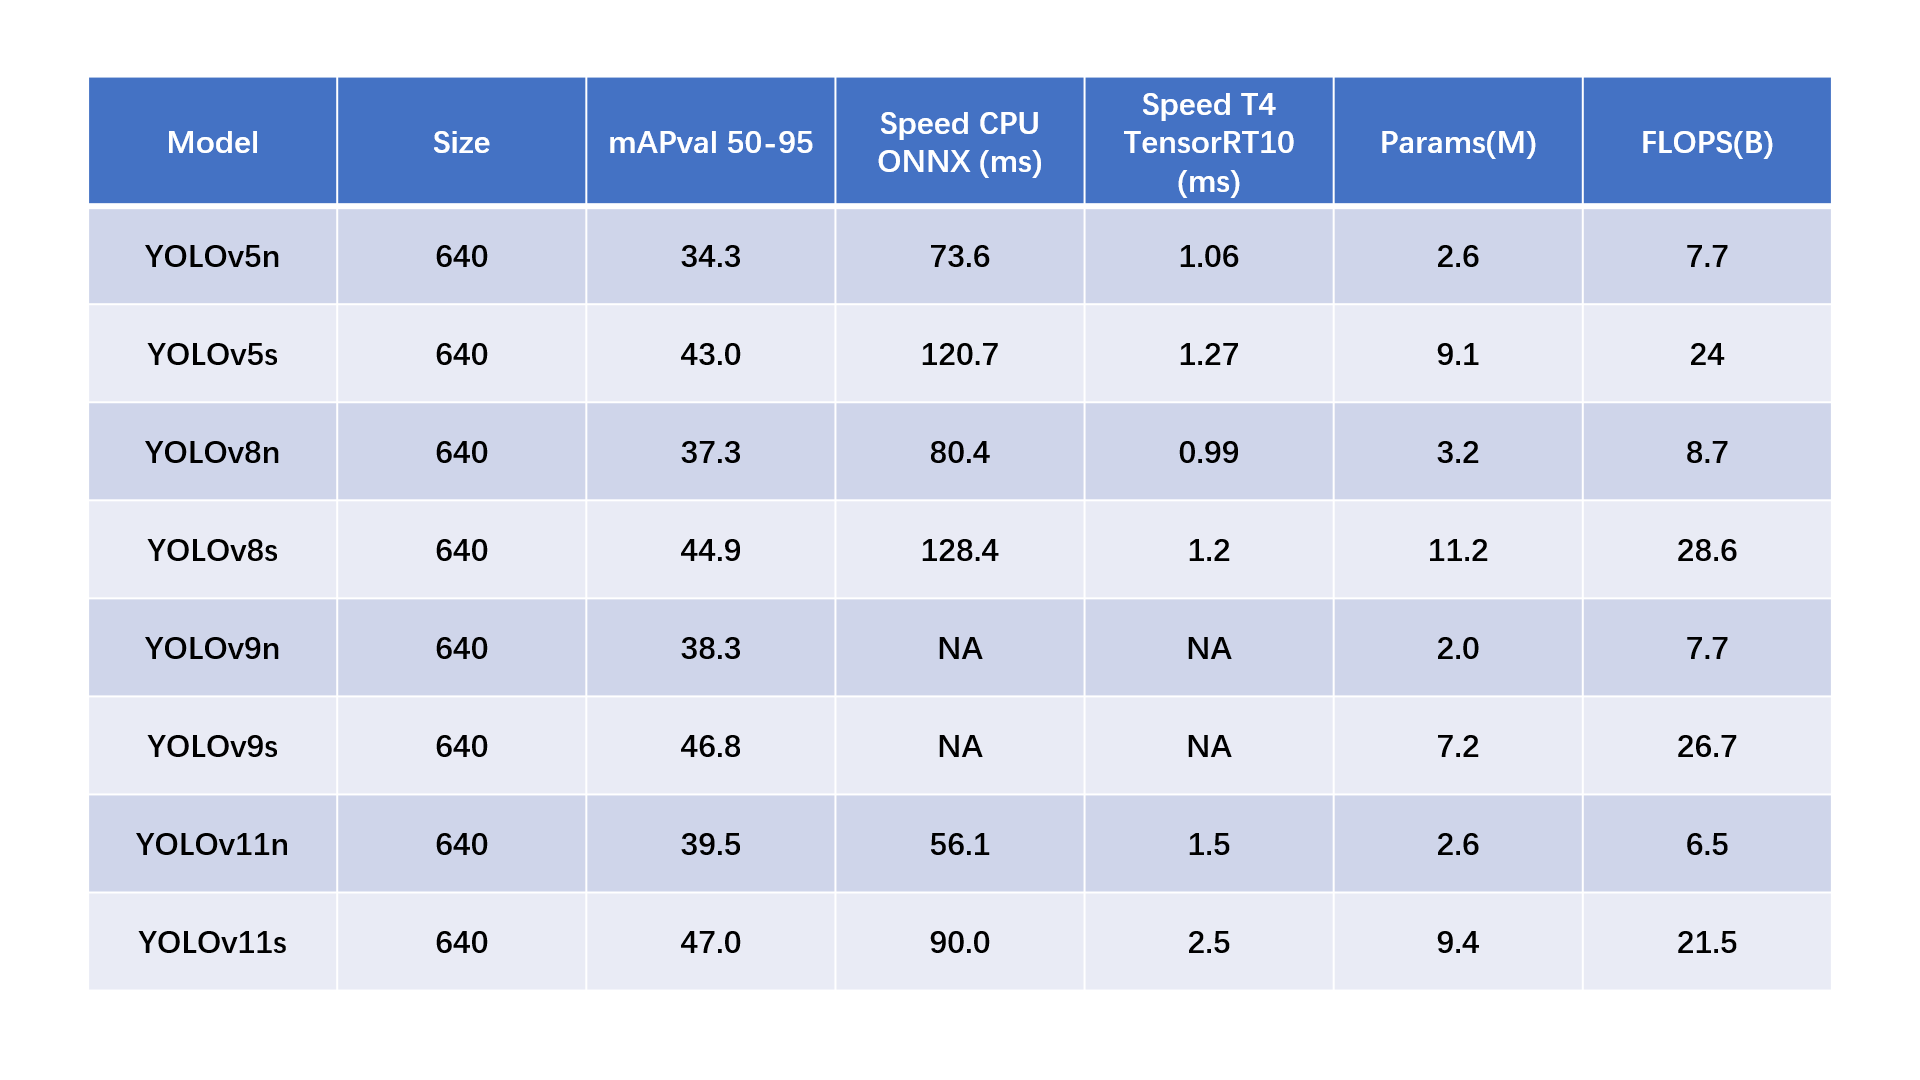
\includegraphics[width=0.85\textwidth]{figs/chap02/compare.png}
%   \caption{YOLO各版本模型性能对比}
%   \label{fig:compare}
% \end{figure}

\section{数据集预处理}
本文所使用的数据集来源于缅甸真实的交通道路照片,该数据集为公开资源(数据集来源:\url{https://www.cvmart.net/dataSets/detail/627})。首先使用LabelImg工具对数据集进行标注,生成xml格式的标注文件,再转换成YOLO格式的txt标注文件。YOLO所使用的txt标注文件的格式如\ref{tab:format}所示,文件的每一行有五个元素,其中中心点位置由x\_center和y\_center两个参数描述,分别对应于图像宽度和高度的相对比例值;而边界框的尺寸特征则通过width和height两个参数表征,同样表示为相对于图像原始宽度和高度的归一化比例值。上述五元组能够表示某一个类别的目标在图像中的位置。

\begin{table}[htb]
      \centering
      \caption[目标数据]{YOLO数据标注格式\label{tab:format}}
      \begin{tabular}{lrrrr}
          \toprule
          \multicolumn{1}{c}{class} & \multicolumn{1}{c}{x\_center} & \multicolumn{1}{c}{y\_center} & \multicolumn{1}{c}{width} & \multicolumn{1}{c}{height} \\
          \midrule
          5 & 0.18229123 & 0.72314815 & 0.09270814 & 0.19629641 \\
          14 & 0.40755224 & 0.68564817 & 0.05677574 & 0.18796234 \\
          15 & 0.84505233 & 0.61064834 & 0.04947934 & 0.12587944 \\
          \bottomrule
      \end{tabular}
\end{table}


本文的原数据集包含5661张摩托车驾乘人员头盔佩戴情况图像,由于其中某些类别的样本数据非常少,对包含这些标签的原图像进行了图像增强,保证每一个类别至少有100张样本图像。具体的增强方法如\ref{fig:enhance}所示。

\begin{figure}[htbp]
    \centering
    \begin{subfigure}[t]{0.3\textwidth}
        \centering
        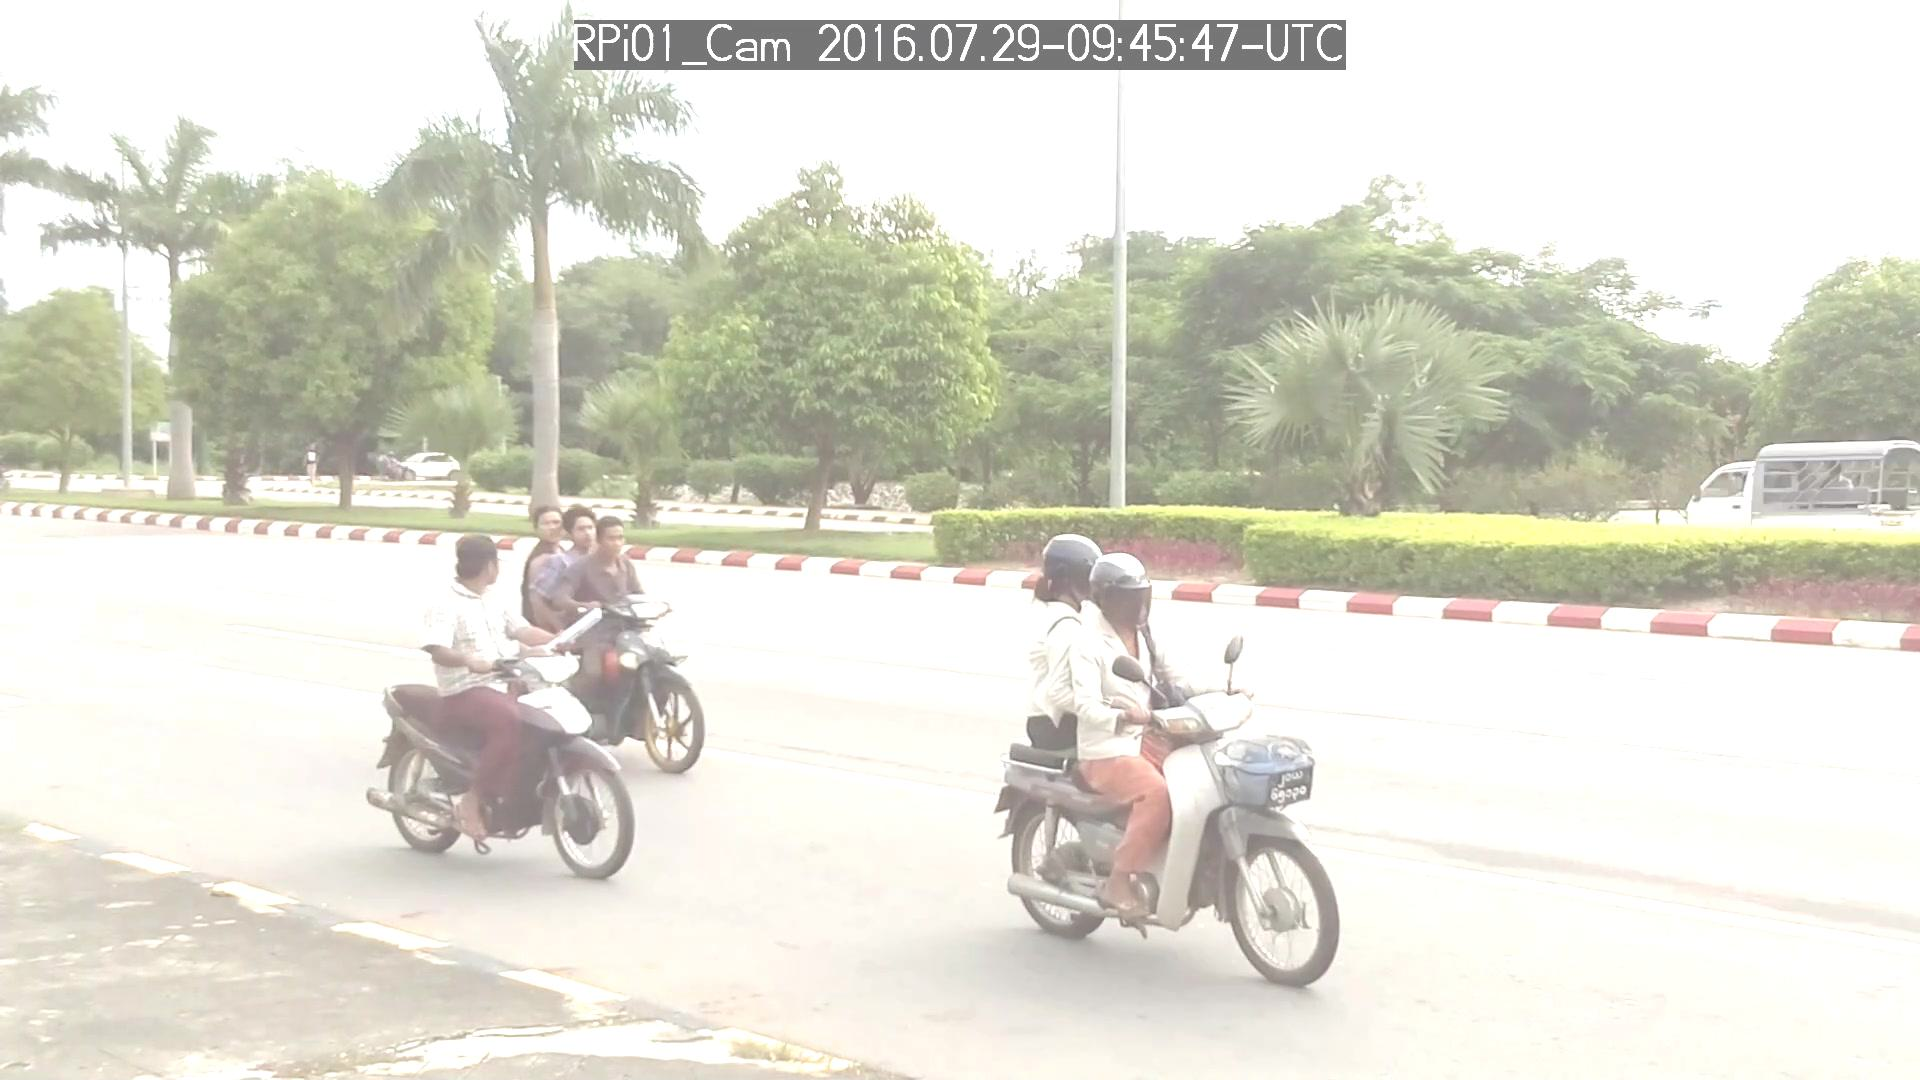
\includegraphics[width=\textwidth]{figs/chap03/rb_origin.jpg}
        \caption{随机亮度}
        \label{fig:sub1}
    \end{subfigure}
    \begin{subfigure}[t]{0.3\textwidth}
        \centering
        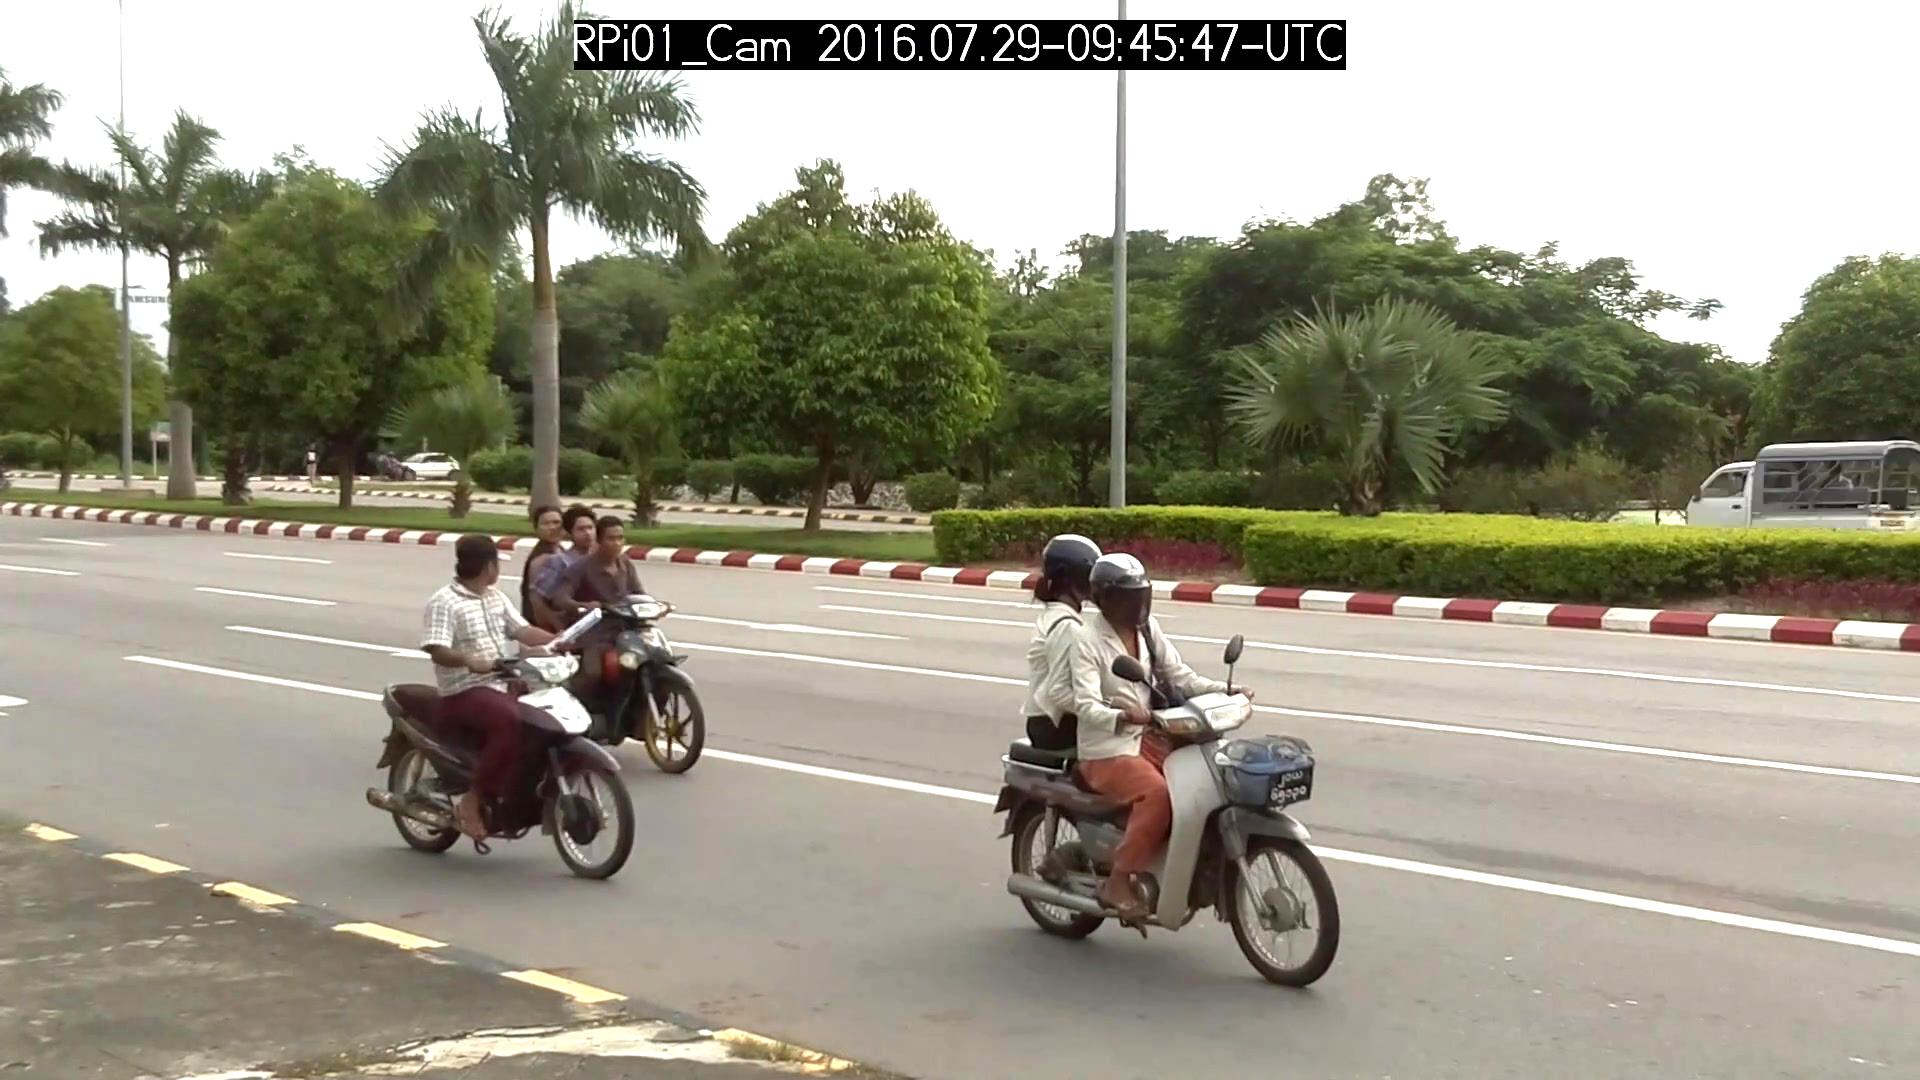
\includegraphics[width=\textwidth]{figs/chap03/rc_origin.jpg}
        \caption{随机对比度}
        \label{fig:sub2}
    \end{subfigure}
    \begin{subfigure}[t]{0.3\textwidth}
        \centering
        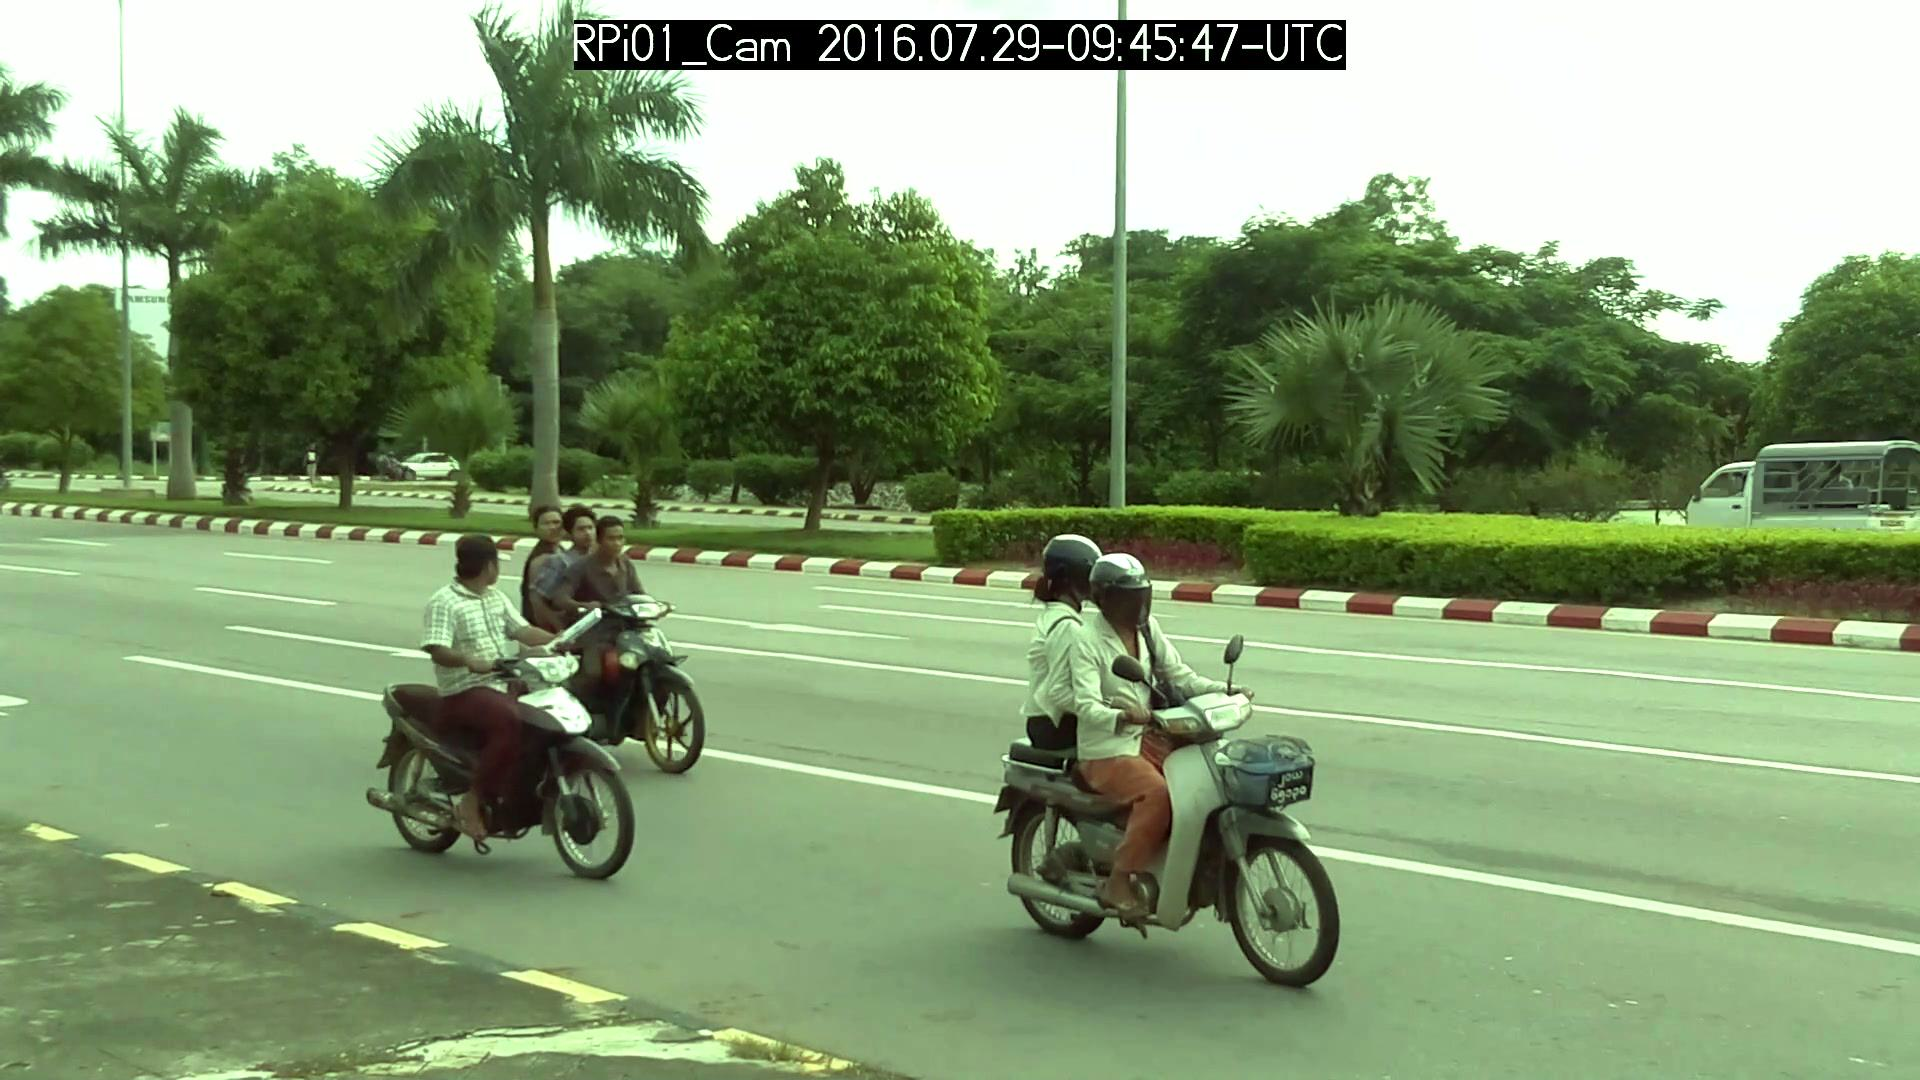
\includegraphics[width=\textwidth]{figs/chap03/rs_origin.jpg}
        \caption{随机饱和度}
        \label{fig:sub3}
    \end{subfigure}

    \begin{subfigure}[t]{0.3\textwidth}
        \centering
        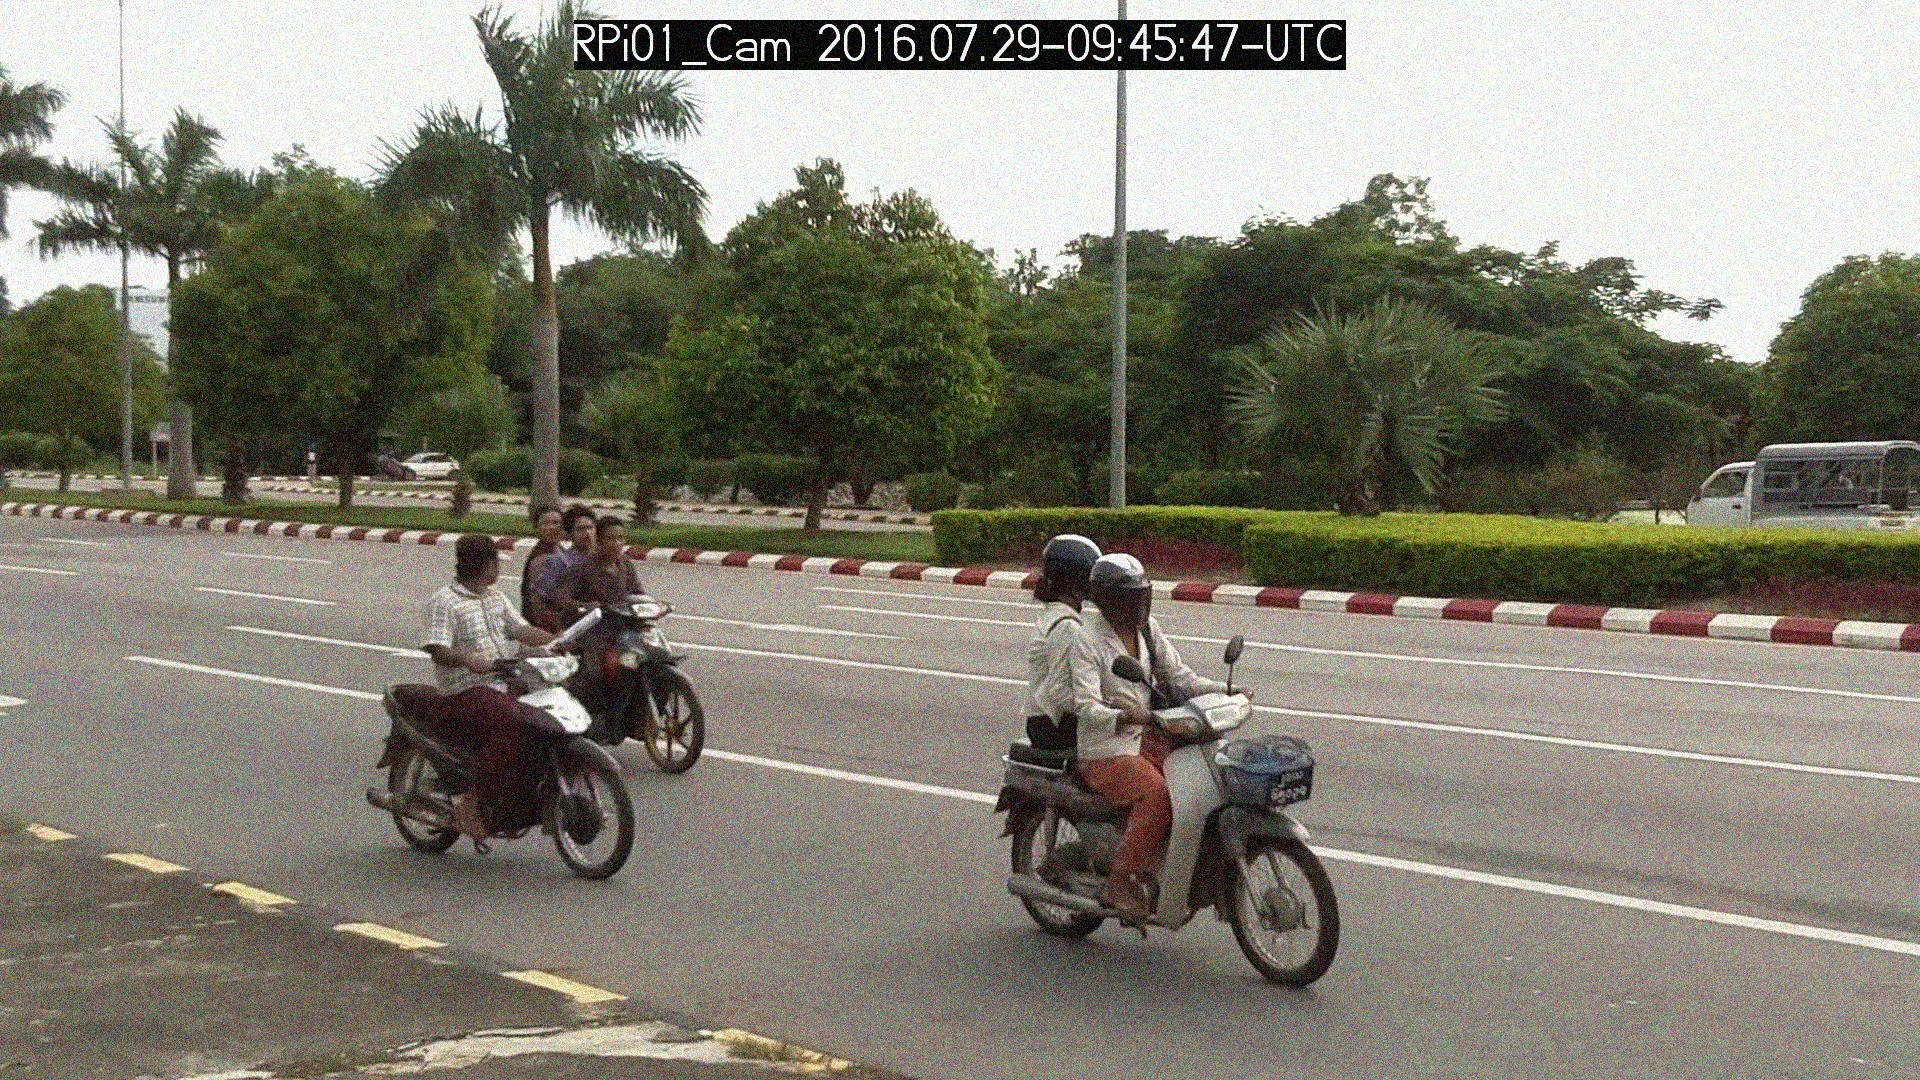
\includegraphics[width=\textwidth]{figs/chap03/gn_origin.jpg}
        \caption{高斯噪声}
        \label{fig:sub4}
    \end{subfigure}
    \begin{subfigure}[t]{0.3\textwidth}
        \centering
        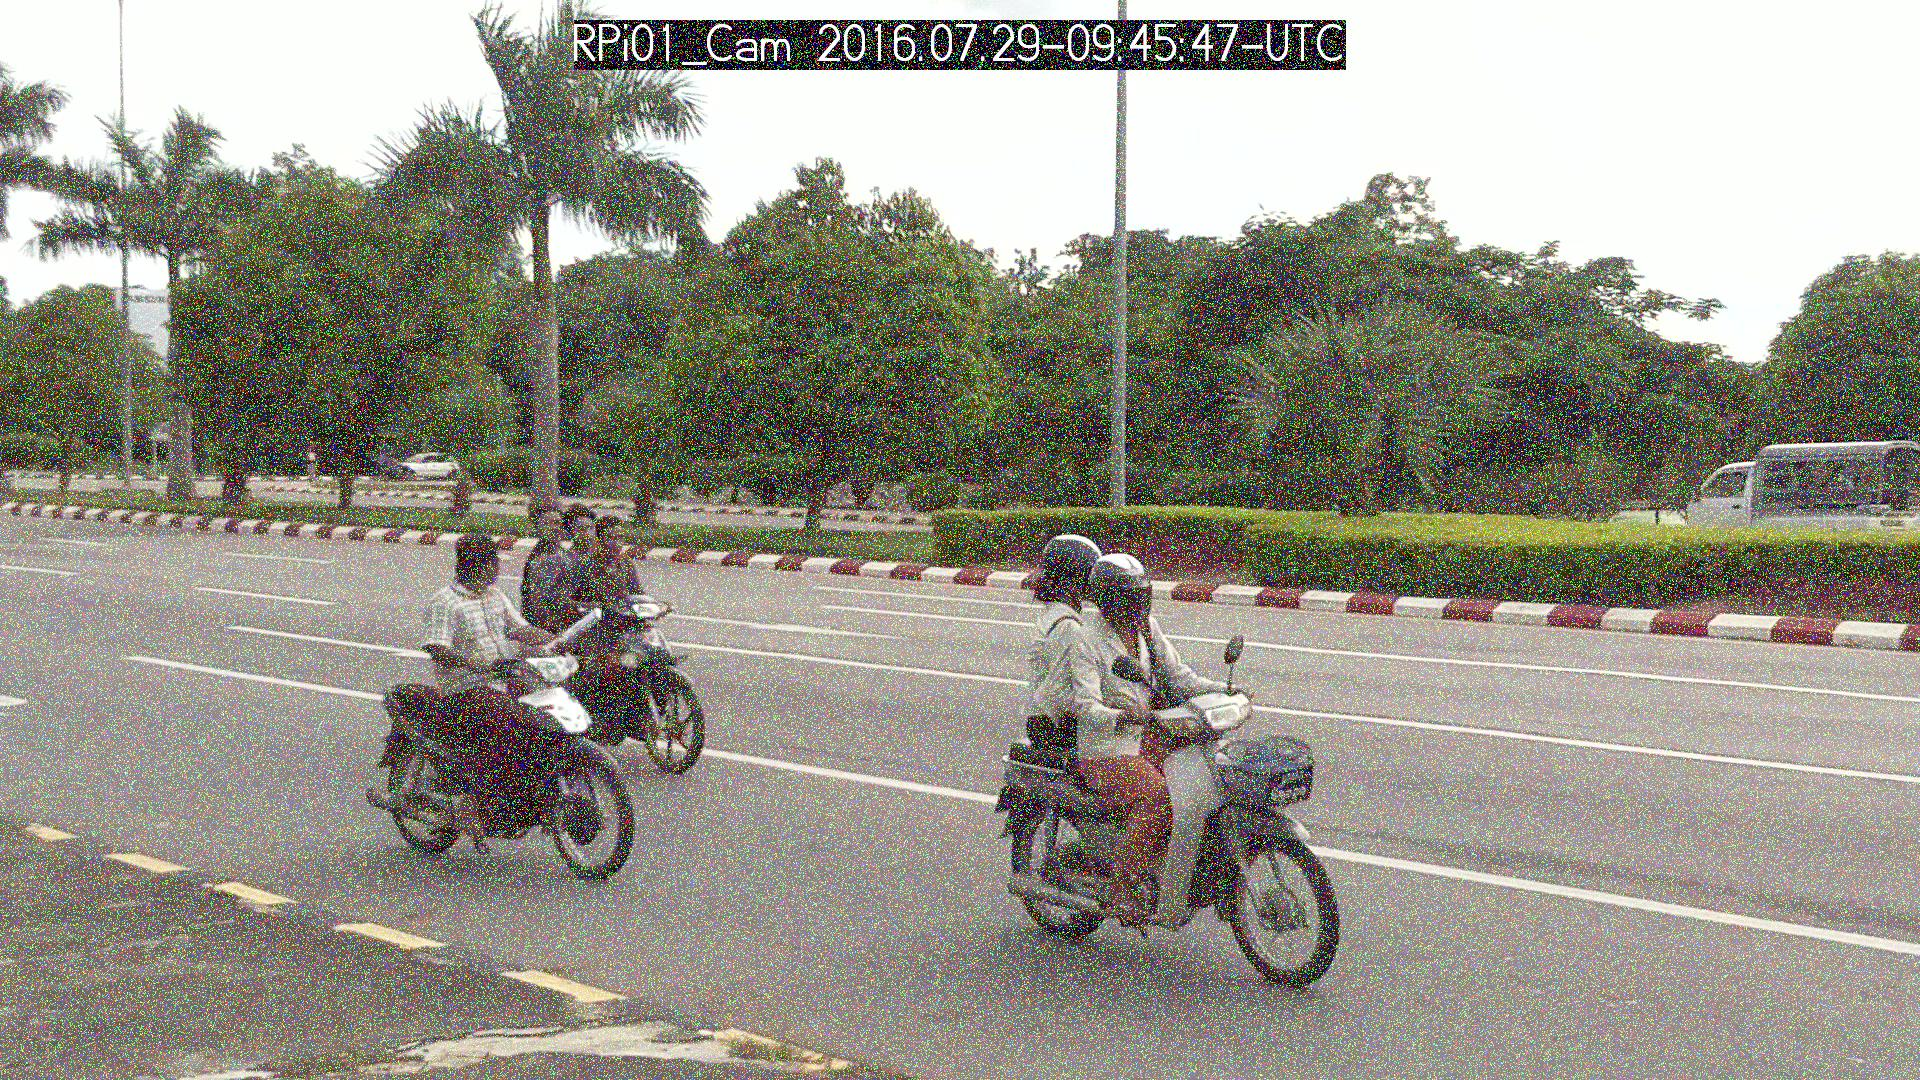
\includegraphics[width=\textwidth]{figs/chap03/sn_origin.jpg}
        \caption{salt噪声}
        \label{fig:sub5}
    \end{subfigure}
    \begin{subfigure}[t]{0.3\textwidth}
        \centering
        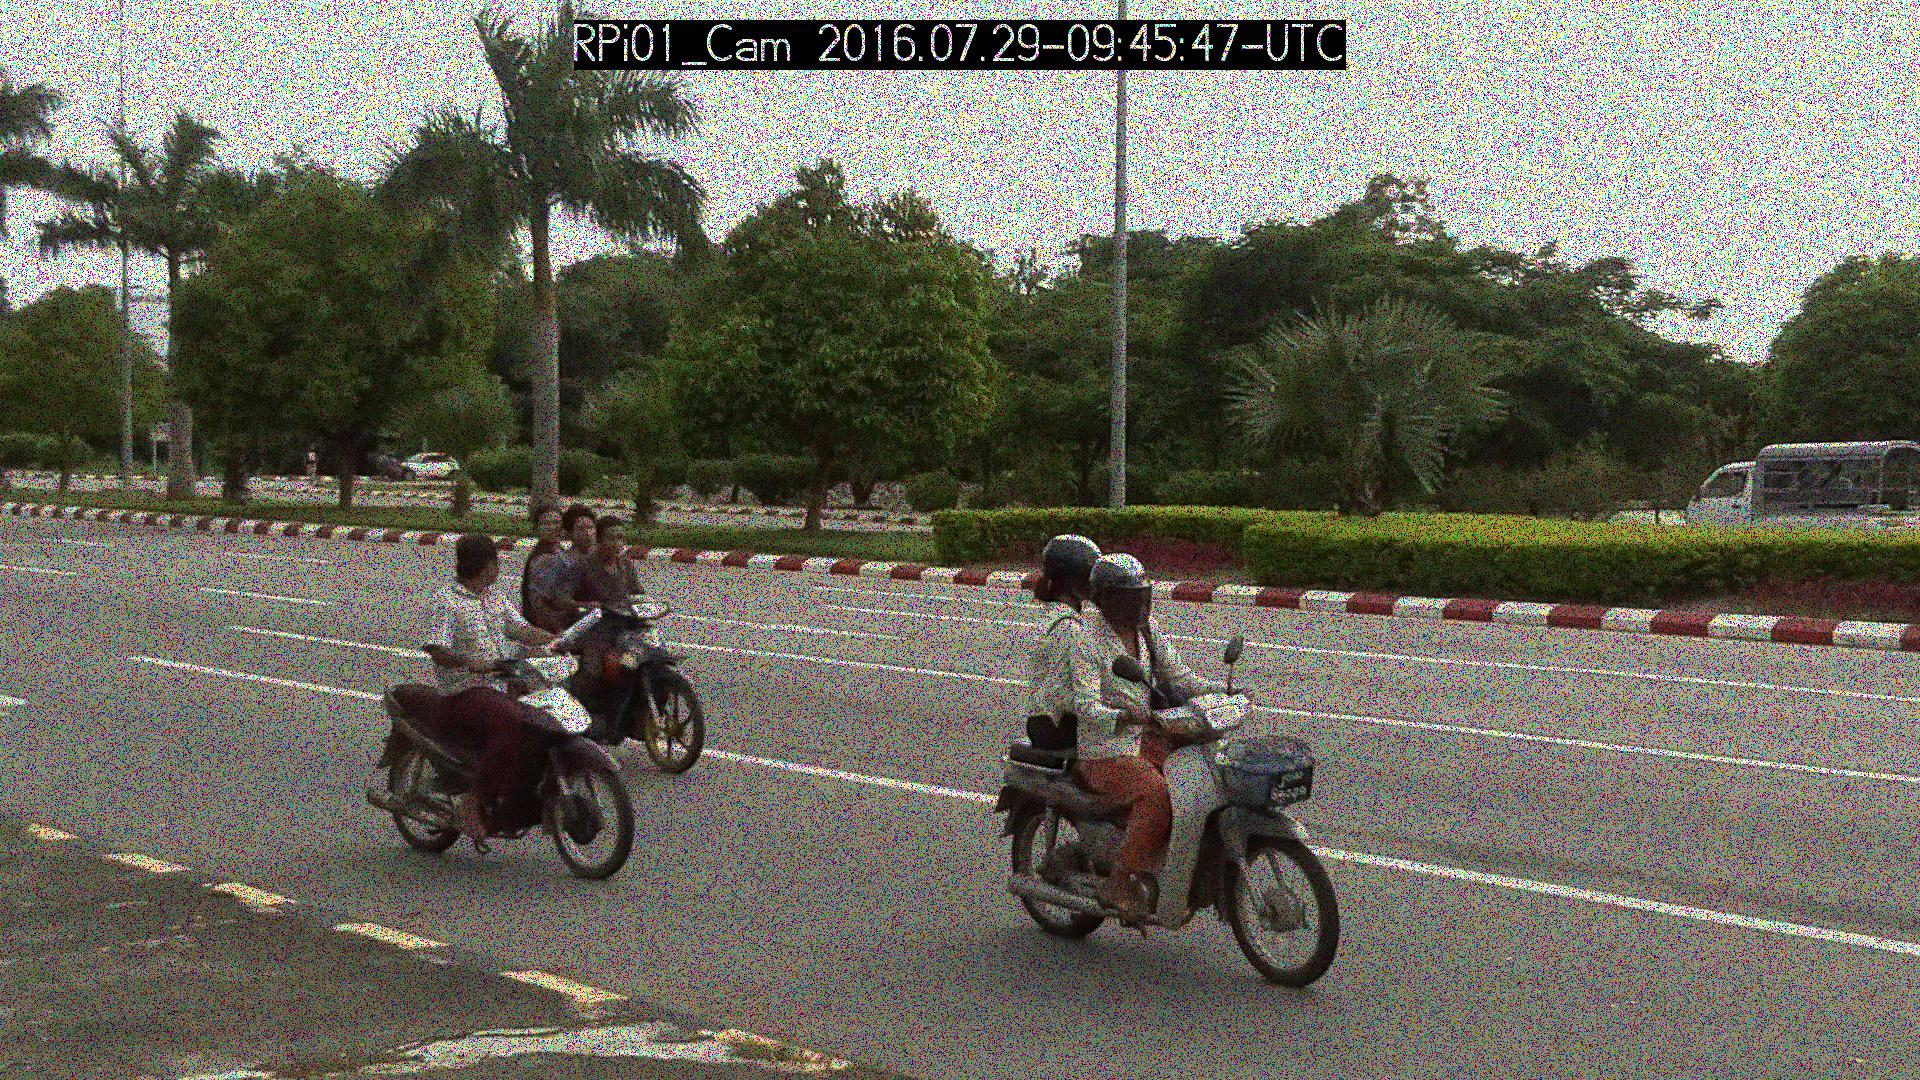
\includegraphics[width=\textwidth]{figs/chap03/pn_origin.jpg}
        \caption{pepper噪声}
        \label{fig:sub6}
    \end{subfigure}
    \caption{图像增强方式}
    \label{fig:enhance}
\end{figure}

对原数据集进行增强之后,共有6282张图像,采用7:2:1的比例对数据集进行随机划分,分别构建训练集、验证集和测试集。本文将目标类别分为18类,标签为S01-S18,其对应关系以及含义如\ref{tab:newlabel}所示,其中meaning一列命名规则为:D(Driver)代表摩托车驾驶员,P(Partner)代表乘车人员。P1代表驾驶员身后的一名乘车人员,P2代表驾驶员身后的另一名乘车人员,P0代表驾驶员身前的乘车人员(在原数据集中,某些小朋友会坐在驾驶员身前)。而D、P0、P1和P2后面紧跟着该乘车人员的头盔佩戴情况,Helmet代表已佩戴头盔,NoHelmet代表未佩戴头盔。例如,标签为S09的含义为DNoHelmetP0NoHelmetP1NoHelmet,表示摩托车驾驶员D未佩戴头盔,驾驶员身前的乘车人员P0未佩戴头盔,驾驶员身后的一名乘车人员P1未佩戴头盔。

\begin{table}[htb]
    \centering
    \caption[标签解释]{目标类别标签含义\label{tab:newlabel}}
    \begin{tabular}{lcl}
        \toprule
        \multicolumn{1}{c}{class} & \multicolumn{1}{c}{label} & \multicolumn{1}{l}{meaning} \\
        \midrule
        0 & S01 & DHelmetP1NoHelmetP2NoHelmet \\
        1 & S02 & DNoHelmetP1NoHelmetP2NoHelmet \\
        2 & S03 & DHelmetP0NoHelmetP1NoHelmet \\
        3 & S04 & DNoHelmetP1NoHelmet \\
        4 & S05 & DHelmetP0NoHelmet \\
        5 & S06 & DNoHelmet \\
        6 & S07 & DNoHelmetP1NoHelmetP2Helmet \\
        7 & S08 & DHelmetP1NoHelmet \\
        8 & S09 & DNoHelmetP0NoHelmetP1NoHelmet \\
        9 & S10 & DNoHelmetP1Helmet \\
        10 & S11 &  DHelmetP0NoHelmetP1Helmet \\
        11 & S12 &  DNoHelmetP0NoHelmetP1NoHelmetP2NoHelmet \\
        12 & S13 &  DHelmetP1NoHelmetP2Helmet \\
        13 & S14 &  DNoHelmetP0NoHelmet \\
        14 & S15 &  DHelmet \\
        15 & S16 &  DHelmetP1Helmet \\
        16 & S17 &  DHelmetP0Helmet \\
        17 & S18 &  DHelmetP1HelmetP2Helmet \\
        \bottomrule
    \end{tabular}
\end{table}

18个类别的样本数量分布如\ref{fig:label1}所示,可以看出S15标签数量最多,共6742个,其表示单一驾驶员佩戴头盔;S06标签数量次之,共6346个,其表示单一驾驶员未佩戴头盔,二者实例数量远高于其他标签。说明单一驾驶员驾驶摩托车是最常出现的情况,且佩戴头盔要比不佩戴头盔的情况稍多一些。除上述两个标签之外,S16和S04是数量最多的两个标签,S16标签共3296个,表示驾驶员和身后的一名乘客都佩戴头盔;S04标签共2503个,表示驾驶员和身后的一名乘客都未佩戴头盔。

由表中数据可以看出,单一驾驶员驾驶摩托车的情况出现次数最多,其次是驾驶员携带一名乘客的情况。并且不管是单一驾驶员,还是驾驶员携带一名乘客,佩戴头盔的情况均多于不佩戴头盔的情况。而一名驾驶员携带一名以上乘客的情况比较少见。

\begin{figure}[!htb]
    \centering
    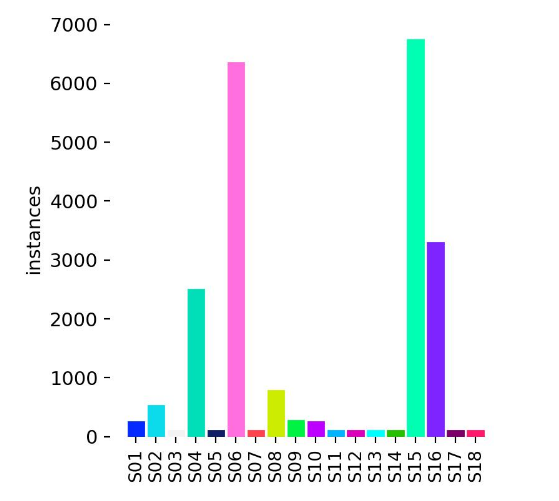
\includegraphics[width=0.8\textwidth]{figs/chap03/label1.png}
    \caption{头盔佩戴情况标签数量分布}
    \label{fig:label1}
\end{figure}

对原数据集5661张图像中的每一个驾驶员目标框进行裁剪,得到33571张包含驾驶员信息的图像,共有570个不同驾驶员。由于驾驶员的图像样本也存在不平衡的情况,对这33571张图像同样进行图像增强,保证每一个驾驶员都至少有100张样本图像。

% \begin{figure}[!htb]
%       \centering
%       \begin{minipage}{0.45\textwidth} % 调整宽度以适应需求,两张图总宽度接近1
%           \centering
%           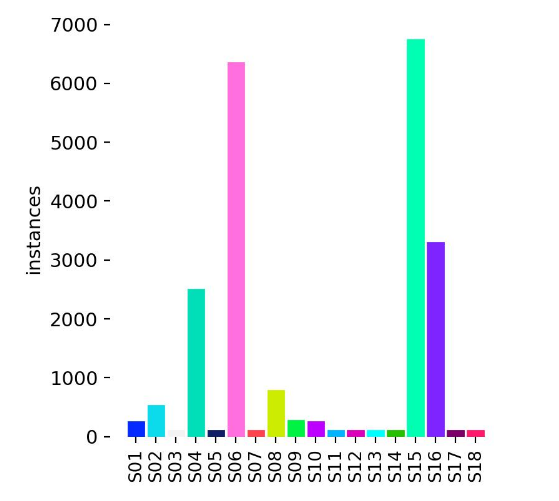
\includegraphics[width=\textwidth]{figs/chap03/label1.png}
%           \caption{头盔佩戴情况标签数量分布}
%           \label{fig:label1}
%       \end{minipage}
%       \hfill % 使两张图像之间保持一定距离
%       \begin{minipage}{0.45\textwidth}
%           \centering
%           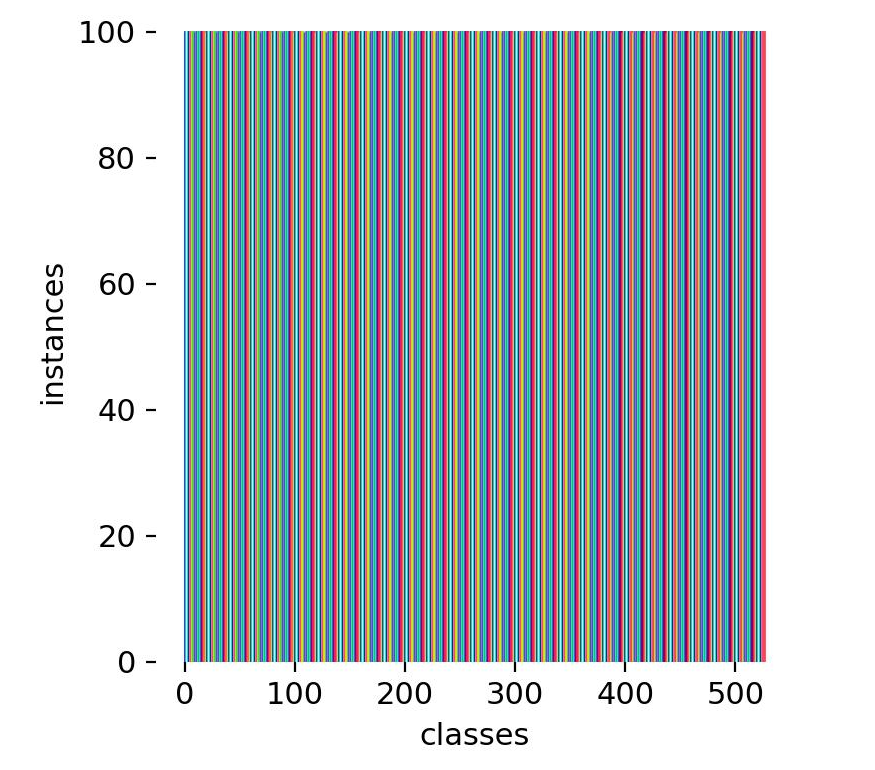
\includegraphics[width=\textwidth]{figs/chap03/label2.png}
%           \caption{驾驶员标签数量分布}
%           \label{fig:label2}
%       \end{minipage}
% \end{figure}

\section{实验环境}
操作系统:Ubuntu 20.04.3 LTS (Focal Fossa)

CPU:Intel(R) Xeon(R) Gold 5318Y CPU @ 2.10GHz

内存:1.5T

GPU:NVIDIA A40

显存:48G

CUDA版本:12.2

Pytorch版本:2.7.0+cu126

\section{参数设置}
本文分别使用YOLOv11n.pt、YOLOv11s.pt、YOLOv11m.pt进行训练,参数设置见\ref{tab:param}。本文进行头盔佩戴情况检测模型训练时,共有18个标签,在yaml文件里nc设置为18。在训练模型中,将batch设置为16,输入图像的size默认设置为640x640,epochs设置为300。
degrees设置为20,在指定度数范围内随机旋转图像,提升模型对摄像头拍摄到的不同角度的图像的识别能力。hsv\_v设置为0.6,将图像的亮度修改一部分,模拟不同的光照环境。translate设置为0.2,将图像进行水平和垂直平移,有助于检测部分可见物体。

\begin{table}[H]
    \centering
    \caption[标签解释]{参数设置\label{tab:param}}
    \begin{tabular}{lll}
        \toprule
        \multicolumn{1}{l}{param} & \multicolumn{1}{l}{value} & \multicolumn{1}{l}{meaing}\\
        \midrule
        nc & 18 & 类别数量\\
        batch & 16 & 训练批次\\
        size & 640x640 & 输入图像的尺寸\\
        epochs & 300 & 训练轮数\\
        degrees & 20 & 控制图像随机旋转的度数范围\\
        hsv\_v & 0.6 & 控制图像亮度调整幅度\\
        translate & 0.2 & 控制图像在水平和垂直方向上的平移程度\\
        \bottomrule
    \end{tabular}
\end{table}

\section{本章小结}
本章首先围绕YOLOv11算法相关理论展开,系统阐述了YOLOv11的网络结构,主要介绍了骨干网络、颈部网络和检测头,说明了YOLOv11对上述三个结构的改进点,并对YOLOv11中三个重要的损失函数做了详细的分析。然后介绍了原数据集的来源和本文使用到的六种数据增强方式,展示了需要训练的两个模型的标签及其数量分布。简要介绍了实验环境以及训练的参数设置。